\begin{frame}{}
  \begin{ffact}{Lex--Monotone Array}
    A \( d \)-dimensional array \( f \) is \textbf{lex--monotone} if there exist
    a permutation \( \sigma : [d] \to [d] \) and signs \( s \in \{-1,+1\}^d \) such that
    \[
      f(x) < f(y) \;\iff\;
      \bigl(s_{\sigma(1)}\,x_{\sigma(1)},\ldots,s_{\sigma(d)}\,x_{\sigma(d)}\bigr)
      <_{\mathrm{lex}}
      \bigl(s_{\sigma(1)}\,y_{\sigma(1)},\ldots,s_{\sigma(d)}\,y_{\sigma(d)}\bigr).
    \]
  \end{ffact}
    \pause
  \smallskip
  Every lex--monotone array is monotone, but not vice versa.
  \smallskip
\end{frame}
\begin{frame}{Types of 2 dimensional lex--monotone arrays}
    \begin{figure}
        \centering
        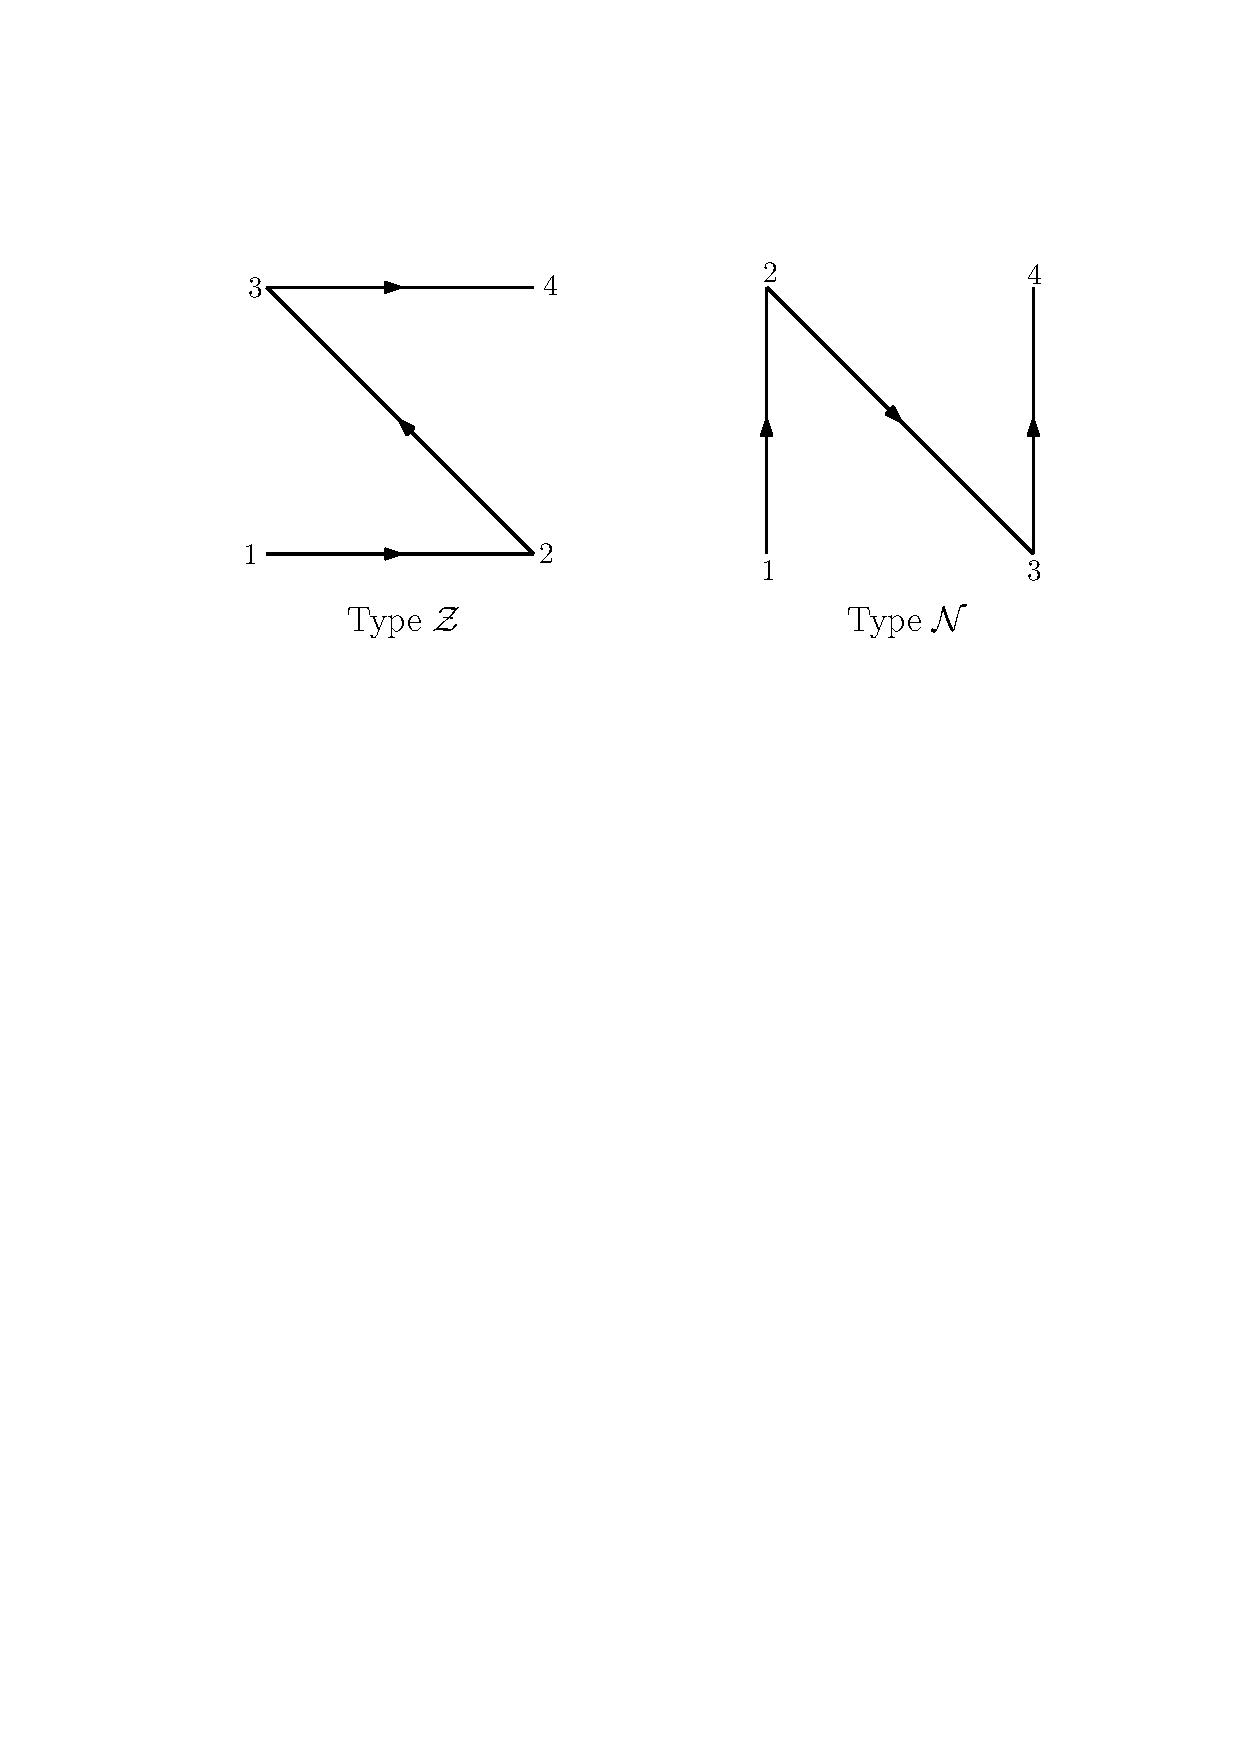
\includegraphics[width=0.9\linewidth]{images/types.pdf}
    \end{figure}
    
\end{frame}
\begin{frame}{Functions \( F_d(n) \) and \( L_d(n) \)}
    \( L_d(n) \): minimum \( N \) such that every \( d \)-dim 
  \( N^d \) array has a lex-monotone \( n^d \) array. \\
  \pause
  \( F_d(n) \): minimum \( N \) such that every \( d \)-dim 
  \( N^d \) monotone array has a lex-monotone \( n^d \) array.
  \pause
  \smallskip
    Obviously \( L_d(n) \leq M_d(F_d(n)) \)\\
    \medskip
    Our proofs work like:
    \vspace{-0.5cm}
\[
\text{Array} 
\xrightarrow{N \geq 2^{2^{n-1}}} 
\text{Inc. monotone}
\xrightarrow{N \geq 2^{O(n^{d-1})}} 
\text{Monotone}
\xrightarrow{F_d(n)} 
\text{Lex--monotone}
\]
\end{frame}
\begin{frame}{\(F_2(n)\leq 2n^2-5n+4\)}
    \begin{columns}
    \begin{column}{0.7\linewidth}
    Let \(f\) be a monotone array \(N^2\), where \(N=(n-1)(2n-3)+1\)\\
    We colour element \((a_i, a_j)\), where \(\set{i,j} \in [1,2n-3]\):
    \begin{itemize}
        \item red if \(f(a_{i+1},a_j)<f(a_i,a_{j+1})\) 
        \item blue if \(f(a_{i+1},a_j)\geq f(a_i,a_{j+1})\) 
    \end{itemize}
    \end{column}
    \begin{column}{0.3\linewidth}
        \begin{figure}
            \centering
            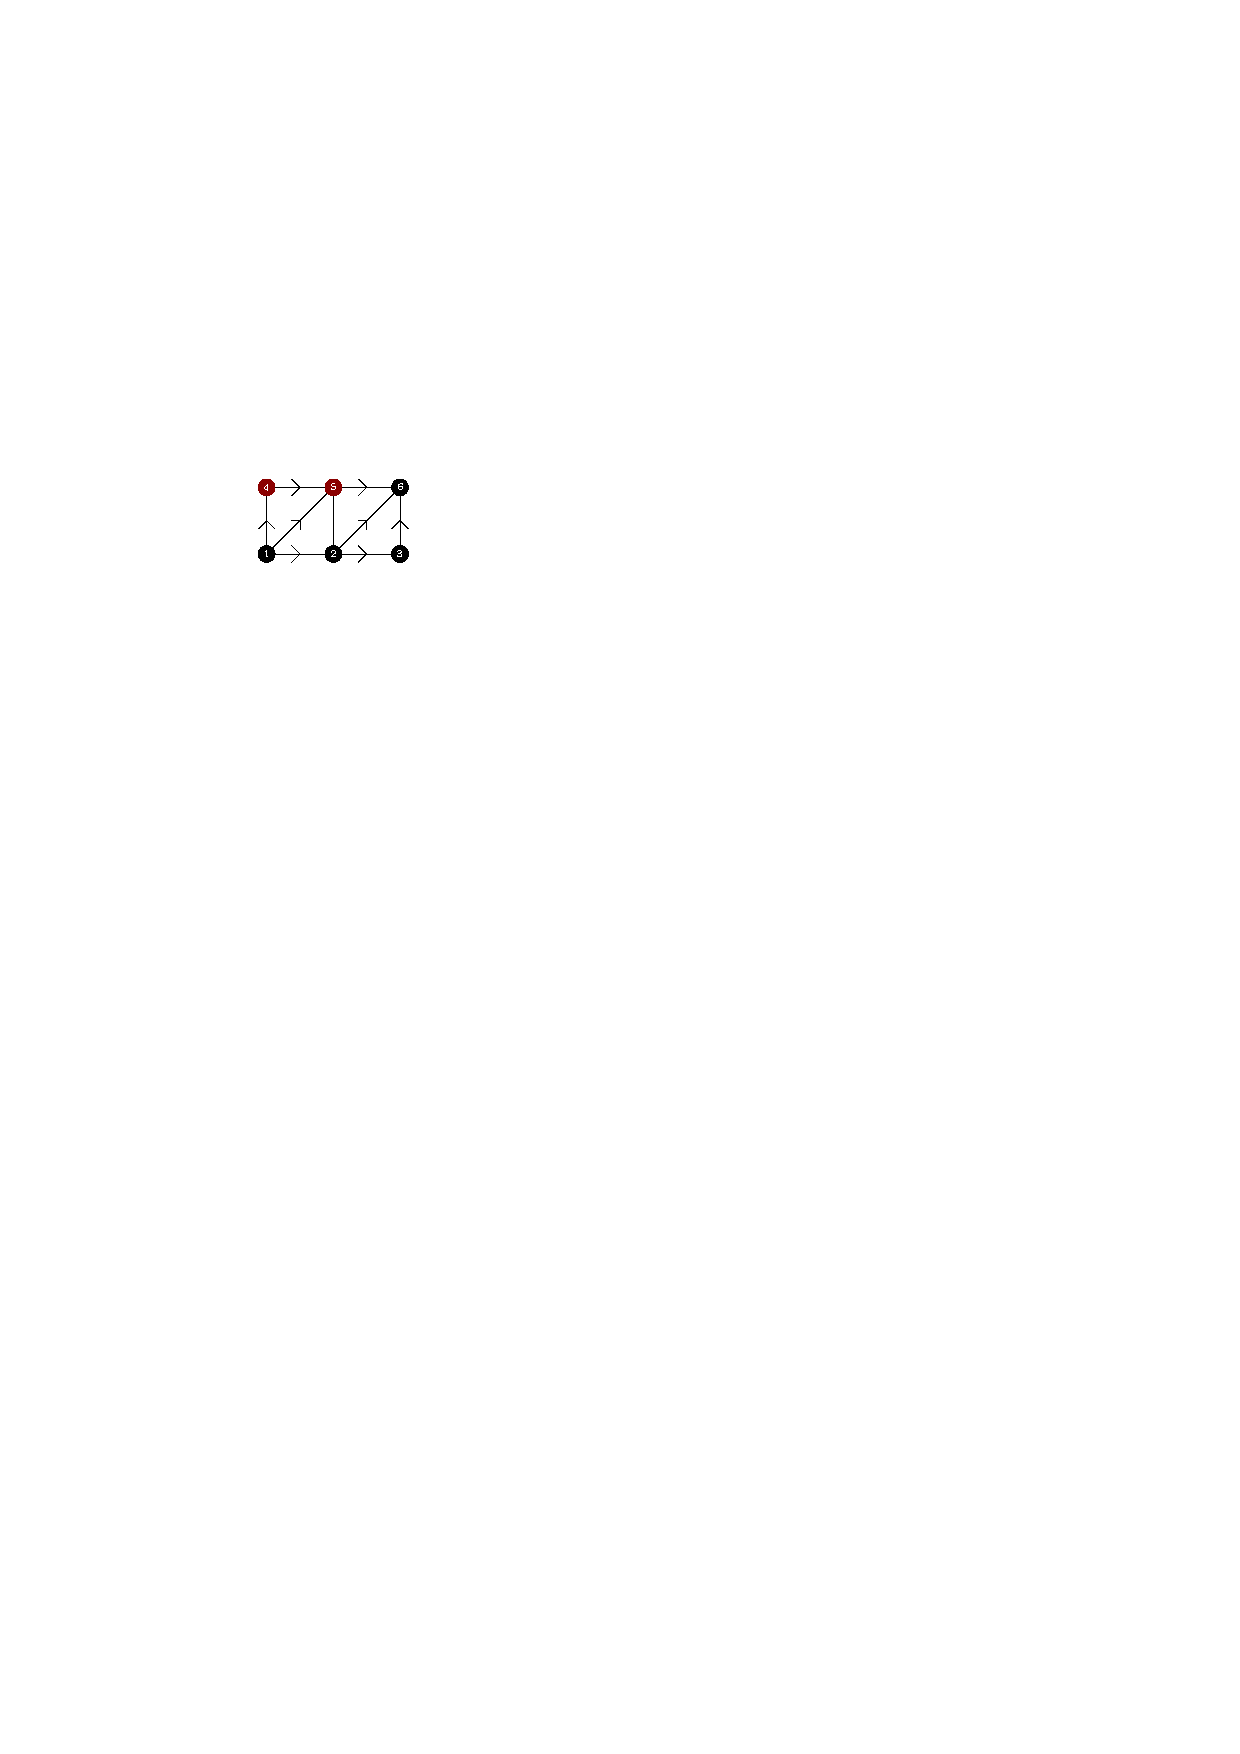
\includegraphics[width=0.8\linewidth]{images/F2.pdf}
        \end{figure}
    \end{column}
    \end{columns}
    \pause
    As \(2(n-2)(2n-3)<(2n-3)^2\) there exists a row with at least \(n-1\) red or a column with \(n-1\) blue points.\\
    \medskip
    Assume there is a row  with red points at \(j_1 < \cdots < j_{n-1}\)
Consider the columns
\vspace{-0.5cm}
\[
j_1,\dots,j_{n-1}, j_{n-1}+1,
\]
\vspace{-0.5cm}\\
Together with rows \(i,i+1\), this forms a \(2\times n\) subarray.\\

By monotonicity these rows and columns yield a type \(\mathcal{N}\) lex--monotone subarray.
\end{frame}

\begin{frame}{}
    \begin{lemma}{Lemma}
        For \(n \geq 3\), there exists an increasing array \(g\) of size \((n-1)(n-2)\times (n-1)^2\) such that
        \begin{itemize}
            \item \(g\) does not contain an \((n-1) \times 2\) subarray of type \(\mathcal{N}\)
            \item \(g\) does not contain an \(n \times 2\) subarray of type \(\mathcal{Z}\)
        \end{itemize}
    \end{lemma}
    \begin{columns}
    \begin{column}{0.5\linewidth}
        \only<1>{
        We take an array \(g\) partitioned into \(C_i\) such that
        \begin{itemize}
            \item \(C_1 < \dots < C_{n-2}\)
            \item Each \(C_i\) is of type \(\mathcal{Z}\).
        \end{itemize}
        }
        \only<2->{
        We can notice that:
        \begin{itemize}
            \item \((n-1) \times 2\) subarray of type \(\mathcal{N}\) would need to intersect in \(2\times 2\) with some \(C_i\), but \(C_i\) is type \(\mathcal{Z}\)
            \only<3>{
            \item \(n \times 2\) subarray of type \(\mathcal{Z}\) would need to intersect two seperate \(C_i\) thus it would contain \(2\times 2\) of type \(\mathcal{N}\)
            }
        \end{itemize}
        }
    \end{column}
    \begin{column}{0.5\linewidth}
        \vspace{-1cm}
        \begin{figure}
            \centering
            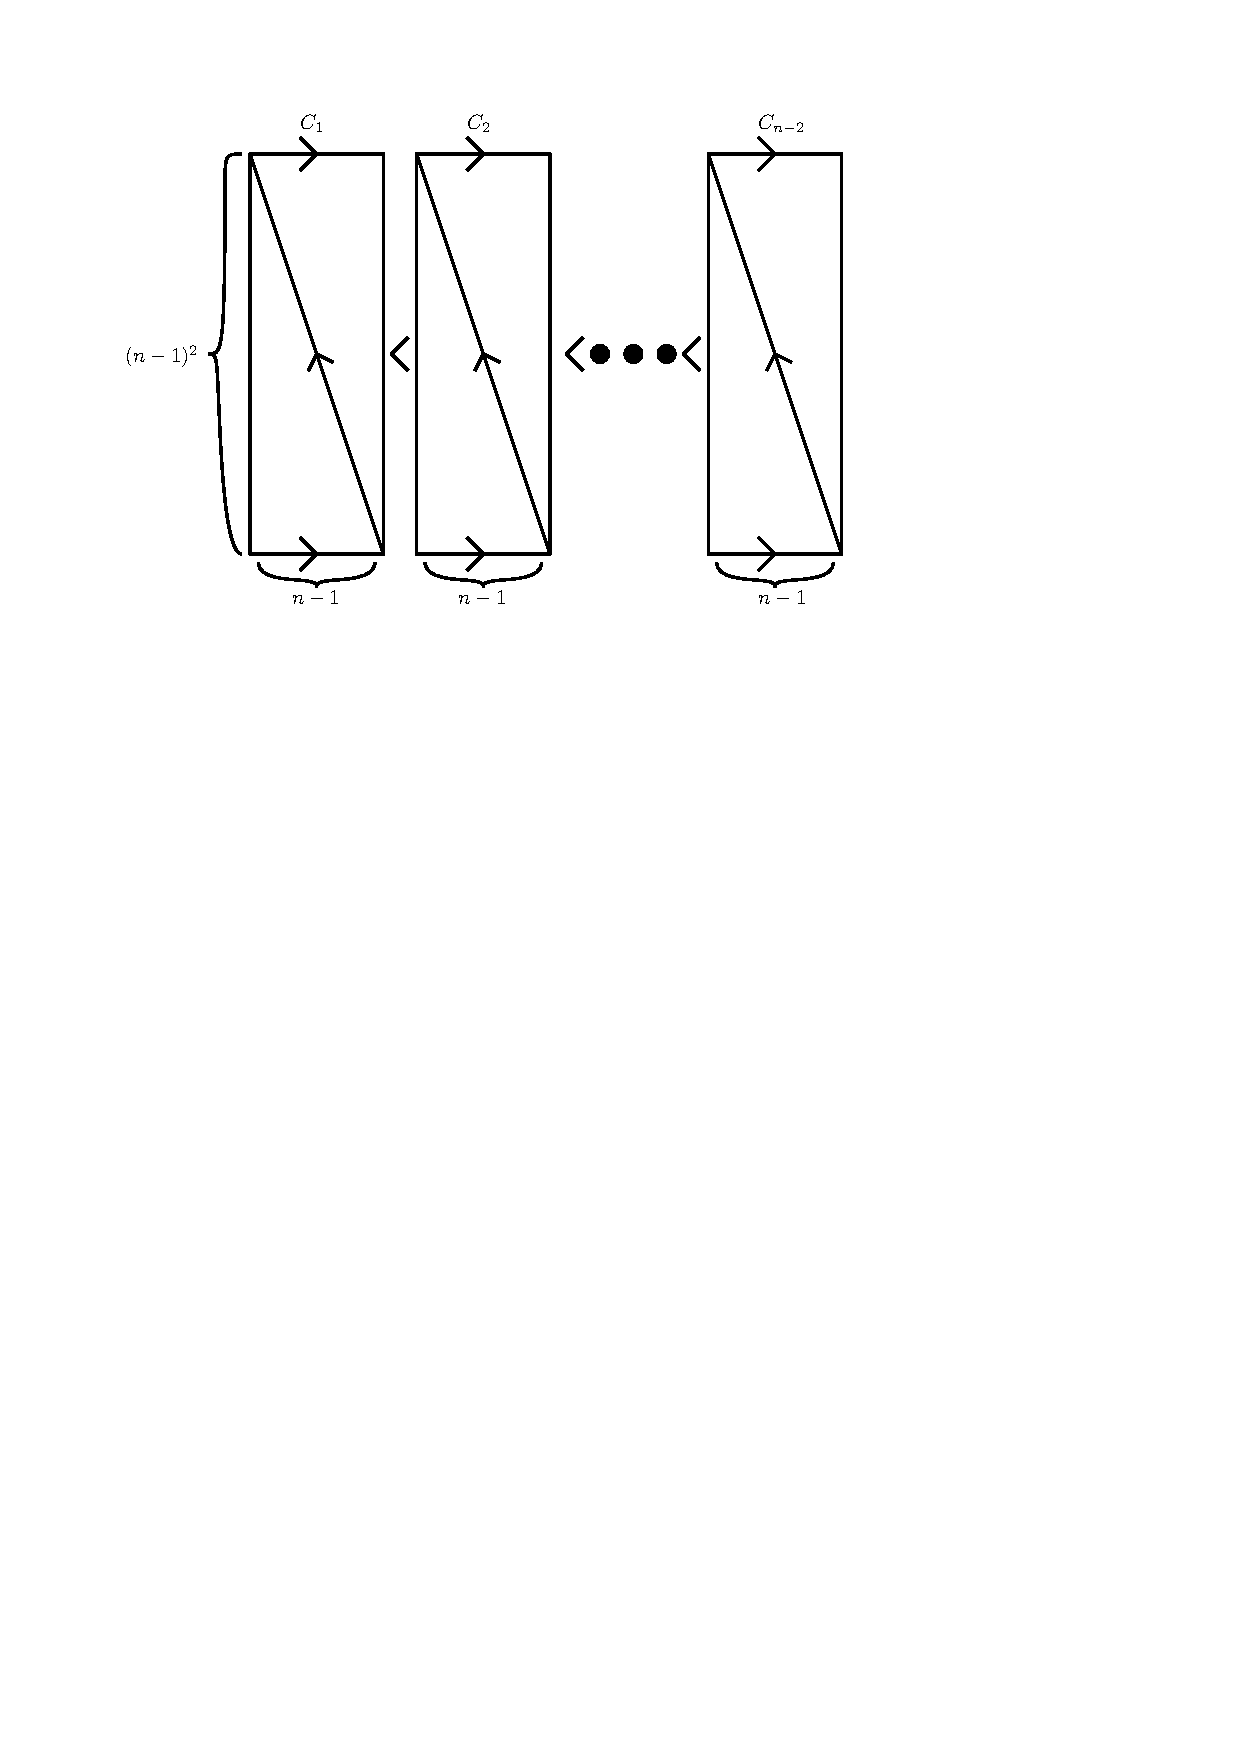
\includegraphics[width=\linewidth]{images/F_2_lower.pdf}
        \end{figure}
    \end{column}
    \end{columns}
\end{frame}


\begin{frame}{}
      \begin{lemma}{Lemma}
        For \(n \geq 3\), there exists an increasing array \(g\) of size \((n-1)(n-2)\times (n-1)^2\) such that
        \begin{itemize}
            \item \(g\) does not contain an \((n-1) \times 2\) subarray of type \(\mathcal{N}\)
            \item \(g\) does not contain an \(n \times 2\) subarray of type \(\mathcal{Z}\)
        \end{itemize}
    \end{lemma}

    \begin{lemma}{Lemma}
        For \(n \geq 3\), there exists an increasing array \(h\) of size \((n-1)^2 \times (n-1)(n-2)\) such that
        \begin{itemize}
            \item \(h\) does not contain an \(2 \times (n-1) \) subarray of type \(\mathcal{N}\)
            \item \(h\) does not contain an \(2  \times N\) subarray of type \(\mathcal{Z}\)
        \end{itemize}
    \end{lemma}
\end{frame}
\begin{frame}{}
    \begin{columns}
    \begin{column}{0.5\linewidth}
        Similarly we can show that if \(N=2n^2-5n+3\) we can construct an \(N\times N\) grid which does not contain an \(n \times n\) subgrid of types \(\mathcal{N}\) nor \(\mathcal{Z}\)\\
        \medskip 
        \begin{proof}{Proof sketch}
                We take 2 copies of \(g\) and two of \(h\) to form an \(n\times n\) grid (we fill the remains with an increasing array)
        \end{proof}
        \medskip
        \only<2>{
        \begin{theorem}{Lower bound}
            \(F_2(n)\geq 2n^2-5n+3\)
        \end{theorem}
        }
    \end{column}
    \begin{column}{0.5\linewidth}
        \begin{figure}
            \centering
            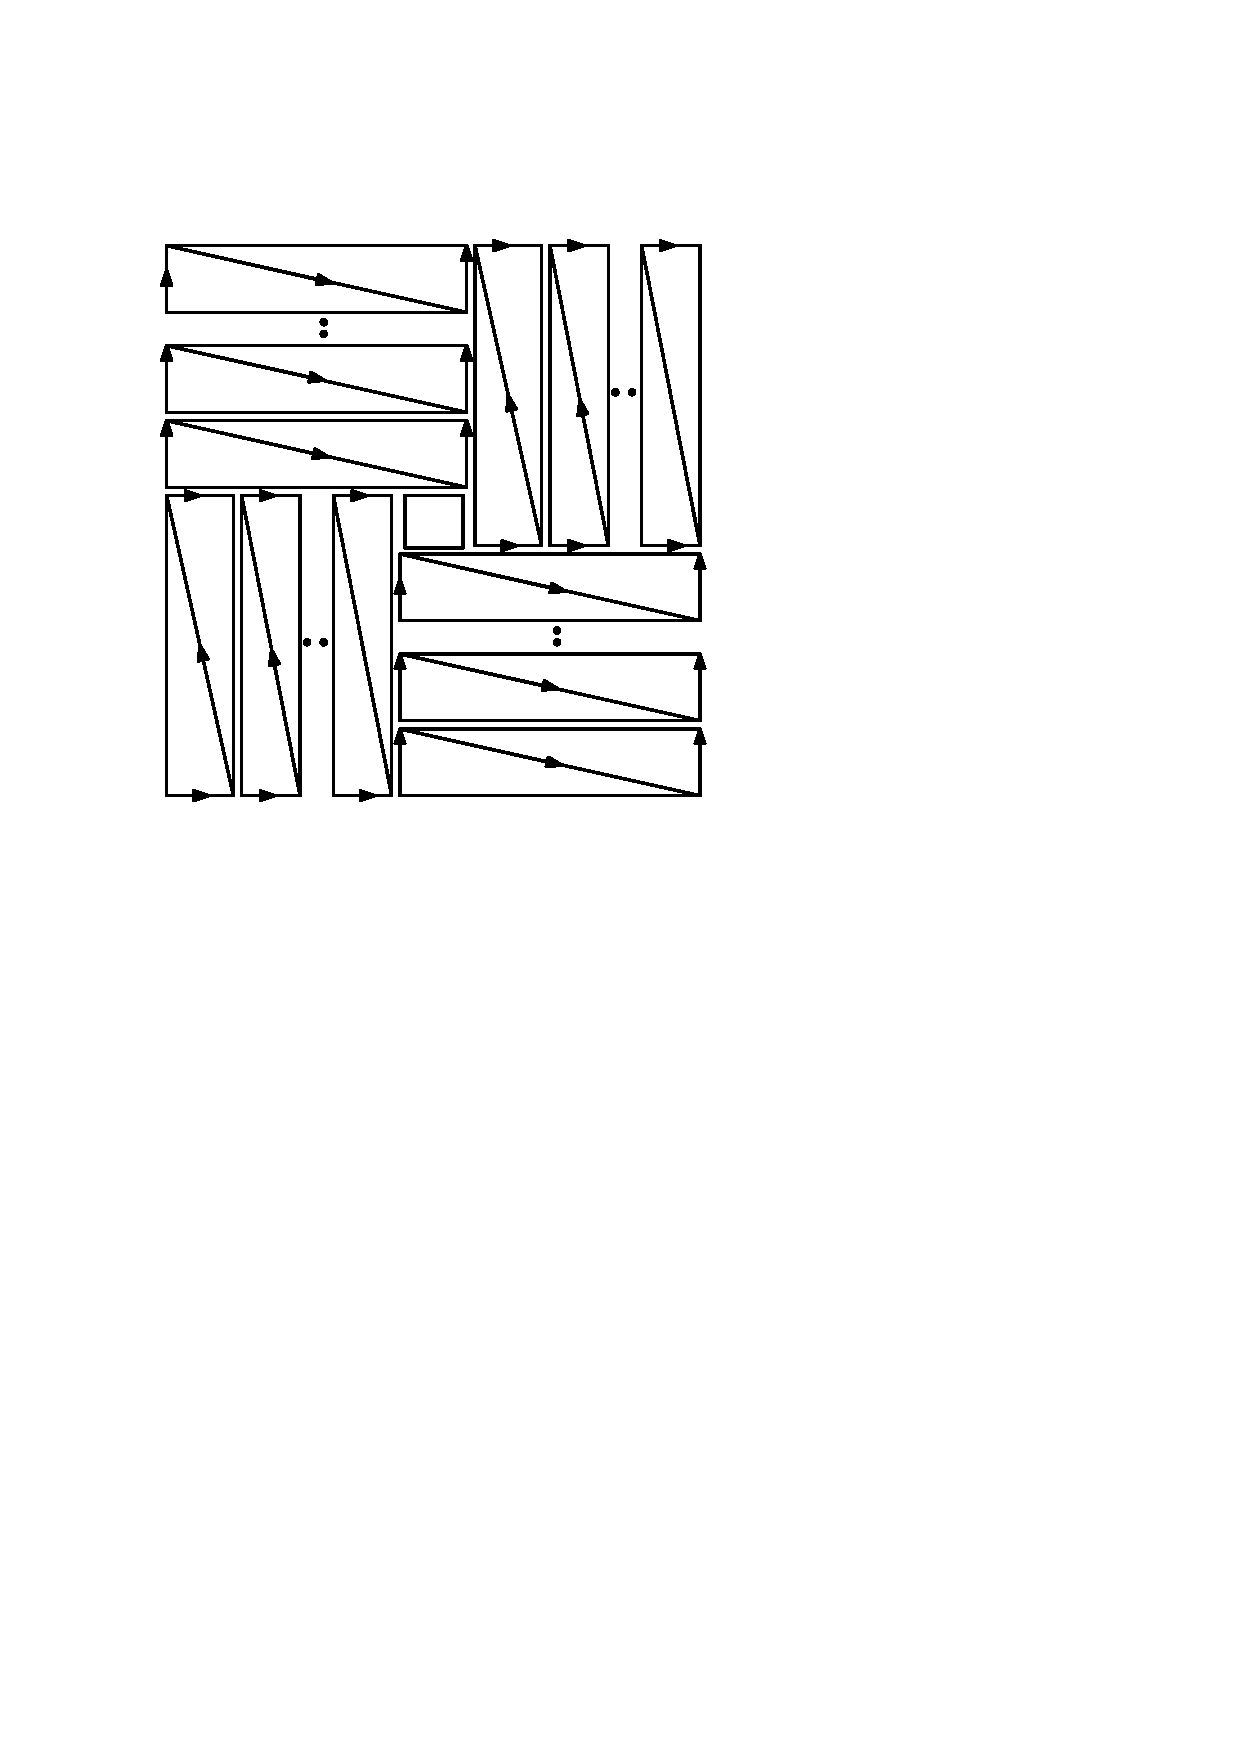
\includegraphics[width=0.8\linewidth]{images/weird.pdf}
        \end{figure}
    \end{column}
    \end{columns}
\end{frame}
\begin{frame}{}
    Through similar idea we can show the bound
    \begin{theorem}{High dimensional bound on \(F\)}
        \[F_d(n)\leq 2^{\left(\frac{1}{2}(d-1)!+o(1)\right)n^{d-2}}\leq 2^{O_d(n^{d-2})}\]
    \end{theorem}
    If we combine it with 
    \begin{theorem}{Bound on \(M_d\)}
        \[M_d(n)\leq 2^{2^{2^{O(n^{d-1})}}}\]
    \end{theorem}
    \pause 
    \begin{theorem}{Bound on $L_d(n)$}
        \[L_d(n) \leq M_d(F_d(n)) \leq 
        \underbrace{2^{2^{2^{O_d\left(2^{O_d(n^{d-2})}\right)}}}}_{\text{quadruple exp}}
        = \underbrace{2^{2^{2^{2^{O_d(n^{d-2})}}}}}_{\text{towr}_5(O_d(n^{d-2}))}\]
    \end{theorem}
\end{frame}

